%                                             -*- coding: utf-8 -*-
% Mindenkinek csak javasolni tudjuk, hogy latex-et használjon.
% Szakdolgozatnál vagy diplománál már egyértelműen kijönnek az
% előnyei a Worddel szemben.  Ennek ellenére ez a sablon messze nem
% tökéletes.  Ha valamit javítanál benne, kérlek, küld vissza, hogy
% hallgatótársaid is profitáljanak belőle.  Köszönöm.

% További nehézséget okoz, hogy a népszerű latex disztribúciók nem
% tartalmazzák a legújabb változatát a magyar.ldf-nek.  A szükséges
% fájlokat a sablon mellé bemásoltuk, de le is tölthetőek innen:
% http://www.math.bme.hu/latex/
%
%
%
\documentclass[a4paper,oneside]{article}
\usepackage[margin=3cm]{geometry}
% =================================================================
% Magyar nyelvi támogatás
%------------------------
% ###################
% Nyelvváltó parancsok:
%\selectlanguage{english}
%\selectlanguage{magyar}
% rövid angol beszúrás:  \foreignlanguage{english}{some english text}
% határozott névelők generálása ``magyar'' babel-el:
% argumentum+megfelelő határozott nevelő: \az{},\Az{}
% csak a megfelelő határozott nevelő: \az*{}, \Az*{}
% címkék: \aref{}, \aref*{}, képletekhez \aref()
%        \Aref{}, \Aref*{}, képletekhez \Aref()
% oldalak: \apageref{}, \apageref*{}
%        \Apageref{}, \Apageref*{}
% idézetek: \acite, \acite*, \Acite, \Acite*
% ###################
\usepackage[english,magyar]{babel} %vegyes nyelvi támogatás a
% magyar helyesírás ellenőrzéshez (ispell) és elválasztáshoz
\selectlanguage{magyar}

%=================================================================
% direkt ékezetes karakter beírás támogatás
%-------------------------------------------
\usepackage[T1]{fontenc}
\usepackage[utf8]{inputenc}
\usepackage{multirow}
%================================================================
% Undorító dolog bitmappelt (Type III) betűtípust nézni a PDF-ben
% képernyőn. Az alapértelmezett Computer Modern font LaTex-ben
% bitmappelt, ezért használjunk Times fontot:
\usepackage{times}

%================================================================
% ha ábrát akarunk beemelni, akkor használjuk a graphicx/graphics
% csomagot és az \includegraphics[width=<width>]{abra.pdf} parancsot
\usepackage{graphicx} %for graphics
%kepek helye a gyokerhez(ehhez a file-hoz kepest) kepest
\graphicspath{{./figs/}}

%================================================================
% Kötelezően használjuk a hyperref csomagot, mert ezzel többek között
%  kultúrált hyperlinkelt PDF-et lehet csinálni az alábbi
%  variációkban, különféle hyperref backend-ekkel:
%  pdflatex,dvipdfm,ps2pdf
% tapsztalataim szerint a MikTeX (Win32) a 'dvipdfm' konverzióval
% optimális  míg a teTeX (Linux/Solaris) jobb szereti a 'dvips' módszert
%------------------------------------
% pontosan egyet kommentezzünk be!!!!!!!
% értelemszerűen backend függően generáljunk dvi-ból PDF-et!!!
%------------------------------------
% A hyperref csomag az utolsó beolvasott csomag legyen, kivéve néhány
% problémás csomagot, pl. algorithm
%-----------
% ########################### FONTOS ###########################
% A hyperref hibásan működik a babel csomag 'magyar.ldf' fájljának
% 1.5-ös verziójánál korábbi változatával. 2004. februárjában a MikTeX
% és teTex disztribúciók még csak a v.1.4 verziót tartalmazták! A fájl
% aktuális verziója a BME Matematikai intézet LaTeX honlapjáról
% elérhető: http://www.math.bme.hu/latex/
% A lusták kedvéért a jelen sablon mellé is mellékelem:
% magyarlatex_0.01-2.tar.gz
% ########################### FONTOS ###########################
%-----------
\usepackage[colorlinks=true]{hyperref}

%%%%%%%%%%%%%%%%%%%%%%%%%%%%%%%%%%%%%%%%%%%%%%%%%%%%%%%%%%%%%%%%%%%
% Itt kezdődik maga a dokumentum
%%%%%%%%%%%%%%%%%%%%%%%%%%%%%%%%%%%%%%%%%%%%%%%%%%%%%%%%%%%%%%%%%%
\begin{document}
%%%%%%%%%%%%%%%%%%%%%%%%%%%%%%%%%%%%%%%%%%%%%%%%%%%%%%%%%%%%%%%%%%%
% Ezt ne piszkáld!!!!
%%%%%%%%%%%%%%%%%%%%%%%%%%%%%%%%%%%%%%%%%%%%%%%%%%%%%%%%%%%%%%%%%%%
\pagestyle{myheadings} % legyen fejléc

\newcommand{\onlabcim}{
  \begin{center}
    \huge{\textbf{Önálló laboratórium beszámoló}}

    \small{Távközlési és Médiainformatikai Tanszék}
  \end{center}
}

% Argumentumok: #1=Név, #2=Neptunkód, #3=szakirány, #4=email, #5 konzulens-1, #6 konzulens-1-email, #7 konzulens-2, #8 konzulens-2-email
\newcommand{\onlabszerzo}[8]{

\begin{center}
  \begin{tabular}{ r l }
  készítette: & \textbf{#1}  \\
              & \href{mailto:#4}{\textbf{#4}}  \\
  neptun-kód: & \textbf{\texttt{#2}}  \\
  ágazat:     & \textbf{#3}  \\
  konzulens: & \textbf{#5}  \\
             & \href{mailto:#6}{\textbf{#6}} \\

  \end{tabular}
\end{center}

}

\lstset{
  basicstyle=\footnotesize\ttfamily,
  showstringspaces=false,
  commentstyle=\color{red},
  keywordstyle=\color{blue}
}

% % Argumentumok: #1=Név, #2=email
% \newcommand{\konzulens}[2]{
%   \noindent\textbf{Konzulens:} #1
%   \newline\emph{Email cím:}\/ \href{mailto:#2}{#2}
%   \newline
%
% }

% Argumentumok: #1=Tanév (xxxx/xx alakban, #2=félév (pont nélkül)
\newcommand{\tanevfelev}[2]{
  \large\noindent\textbf{Tanév:} #1. tanév, #2. félév
  \newline
}

% Argumentumok: #1=téma címe
\newcommand{\feladatcim}[1]{
  \large\noindent\textbf{Téma címe: #1}
  \bigskip
}

% Argumentumok: #1=téma részletei
\newcommand{\feladatmaga}[1]{
\large\noindent\textbf{Feladat:}
  \newline
 #1
 \newline
 \smallskip
}

% A fejezetek közé beágyazott irod.jegyzék
\def\thebibliography#1{\renewcommand{%
\baselinestretch}{1}\subsection{A tanulm\'anyozott irodalom jegyz\'eke}\list
 {\small [\arabic{enumi}]}{\settowidth\labelwidth{[#1]}\leftmargin\labelwidth
 \advance\leftmargin\labelsep
 \usecounter{enumi}}
 \def\newblock{\small \hskip .11em plus .33em minus .07em}
 \sloppy\clubpenalty4000\widowpenalty4000
 \sfcode`\.=1000\relax}
\let\endthebibliography=\endlist%


%%% Local Variables:
%%% mode: latex
%%% TeX-master: "template"
%%% End:
 % Ez kell!!!
\markright{Váradi Richárd Tamás (XA5OZH)} % egyoldalas fejléc!!!
%--------------------------------------------------------------------
% fedlap
%--------------------------------------------------------------------
\begin{titlepage}
%bme logo
 \begin{figure}[h]
    \centering
      
\includegraphics[width=12cm]{bme_logo}
  \label{fig:bme_logo}
  \end{figure}
  \thispagestyle{empty}
  %cím generálás
  \onlabcim

% \begin{center}
%   \begin{tabular}{ p{3cm} p{5cm} }
%
%   Készítette: & Beszámoló Péter  \\
%   Neptun-kód: & BPOX43  \\
%   Ágazat: & Médiainformatika  \\
%   E-mail cím: & b.peter@onlab.hu  \\
%   Konzulens: & Dr. Péhádes István  \\
%   E-mail cím: & pehades@tmit.bme.hu  \\
%   Konzulens: & Doktor Andusz  \\
%   E-mail cím: & doktora@tmit.bme.hu  \\
%
%   \end{tabular}
% \end{center}


  %\szerzo argumentumok: #1=Név, #2=Neptunkód, #3=szakirány, #4=email,#5 konzulens-1, #6 konzulens-1-email, #7 konzulens-2, #8 konzulens-2-email
  \onlabszerzo{Váradi Richárd Tamás}{XA5OZH}{Médiainformatika}{ricsi19981007@gmail.com}{Dr. Rétvári Gábor}{retvari@tmit.bme.hu}{}{}


%\feladatcim argumentuma a feladat rövid, 1 soros címe
  \feladatcim{A Kubernetes és a szolgáltatáshálók hálózati kérdései}

  %\feladatmaga argumentuma a feladat 1-2 bekezdésnyi ismertetése
  \feladatmaga{A Kubernetes és szolgáltatáshálók hálózati megoldásainak feltérképezése volt.
  Az egyik olyan probléma, amit én és a konzulensem találtunk, hogy az Istio, mint szolgáltatásháló
  nem képes UDP (User Datagram Protocol) csomagok fogadására. Viszont az Istio-ban használt Envoy proxy
  egy újabb verziója már képes UDP csomagokat továbbítani így megvalósítható az is, hogy az Istio-ba
  ilyen forgalmat irányítsunk be. A félév során egy olyan megoldást kellett találnom, amivel az Istio elé
  ezzel a proxy-val képes legyek egy úgynevezett átjárót létrehozni. Ennek az átjárónak UDP csomagokat kell
  tudnia fogadni és átalakítani őket olyan formátumúvá, amit az Istio képes lekezelni. }


  %\tanevfelev argumentumok:
  % #1=Tanév (xxxx/xx alakban), #2=félév (pont nélkül!)

  \tanevfelev{2019/20}{II}

\end{titlepage}

%==================================================================
\section{A laboratóriumi munka környezetének ismertetése,
     a munka előzményei és kiindulási állapota}
\label{sec:kornyezet}
% A munka  előzményei és kiindulási állapota
% \newpage
\subsection{Bevezető}
\label{sec:bevezeto}
Az ötlet alapvetően egy GitHub-os hibajegyből született. A GitHub egy
webalapú verziókezelő és együttműködésű felület szoftverfejlesztőknek.
A hibajegyek úgy születnek, hogy projektekhez lehet őket hozzáírni és erre jó
eséllyel a fejlesztők vagy más felhasználók reagálnak. Számunkra most ez a jegy
lesz a fontos: \url{https://github.com/istio/istio/issues/1430}. Pár példát szeretnék
idézni és fordítani, hogy miért kellene ez a támogatottság:
\begin{itemize}
	\item  Publikus felhők, ahol egy titkosított szolgáltatáshálót hoznának létre, amely
	képes kezelni olyan dolgokat, mint a DNS (Domain Name System) és NTP (Network Time Protocol).
	\item IoT (Internet of Things) területen.
	\item Telekommunikáció terén is jó lehet a 3G-től használják az UDP protokollt adattovábbításra.
\end{itemize}
Ennek megvalósítására a konzulensemmel úgy gondoltuk, hogy érdemes lenne
egy átjárót felépíteni az Istio elé, amelyet az alábbi ábrákon be is mutatok.
\begin{center}
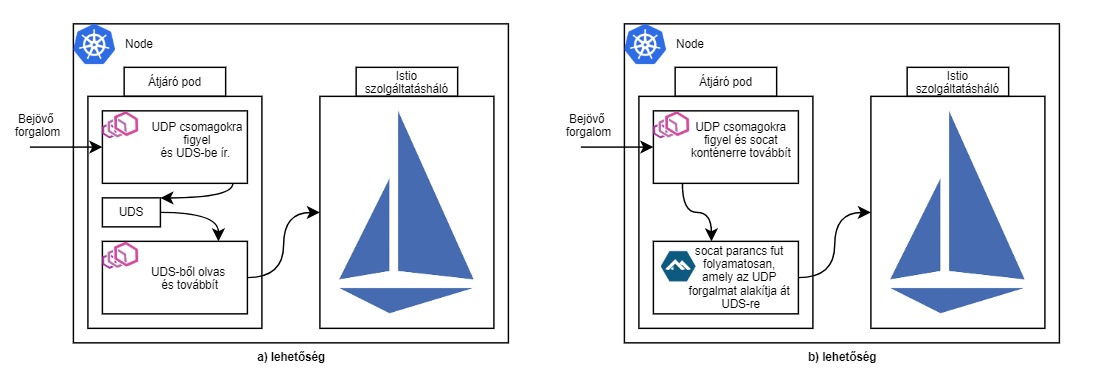
\includegraphics[width=\textwidth]{teljes_architektura}
\end{center}
Az \textbf{a} lehetőség nem teljesen biztos, hogy megvalósítható az Envoy korlátai
miatt. Az Envoy egy nyílt forráskódú perem és szolgáltatás proxy, ami natív felhőalkalmazásokhoz
lett írva C++-ban. Ez a megvalósítás elméleti szinten működőképes lenne,
viszont nagyon kevés dokumentáció található arról, hogy az UDS (Unix Domain Socket)
pontosan hogyan működik az Envoy-ban. \\
A \textbf{b} megoldás annyiban egyszerűbb, hogy ott kettő konténert hozunk létre egy pod-ban, ahol
az Envoy UDP csomagokat figyel és UDP csomagokat továbbít egy Alpine alapú konténernek, amiben fut egy
socket parancs, ami képes UDP forgalmat UDS-re irányítani. A Pod a kubernetes legkisebb egysége,
amelyekben konténereket lehet létrehozni. A konténereket érdemes úgy létrehozni, hogy
konténerenként egy folyamat fusson benne. Az Alpine egy nagyon kicsi erőforrás igényű Unix alapú
operációs rendszer.
%<Mit kell tudni a feladatról, esetleges elméleti bevezető (nagyon
%értelemszerű dolgokat ne definiáljunk, de jó, ha egy kicsit
%kontextusba kerül a témakör, miért fontos ez nekünk, mi volt eddig,
%milyen megoldások jöhetnek szóba és miért emellett döntöttünk, milyen
%kari nagyobb projektbe kapcsolódik ez), stb. Terjedelem max. 50\%
%beszámolónak.>

%Ennek a résznek az a szerepe, hogy az olvasó számára megmutassa az
%elvégzett munka tágabb környezetét. Ez a rész lehet megegyező tartalmú
%más, ugyanazon a témán dolgozó hallgatókéval, de akkor mindenképpen
%tüntessük fel, hogy kivel dolgoztatok együtt, és hogy pontosan, hogy
%osztottátok meg a munkát.

\subsection{Elméleti összefoglaló}
\subsubsection{Docker}
A Docker egy szolgáltatáskészlet Paas (Platform as a Service) termékcsalád,
amelyek operációs rendszer szintű virtualizációt végeznek, hogy a szoftvert
csomagokban, úgynevezett konténerekben lehessen létrehozni.

A konténerek egymástól elválasztva és saját szoftverüket futtatva léteznek
külön könyvtárakkal és konfigurációs fájlokkal. Ezek a konténerek képesek
kommunikálni egymással jól definiált csatornákon keresztül. Érdemes azt az
elvet szem előtt tartani, hogy minden konténerben csak egyetlen folyamat fusson
így sokkal egyszerűbb esetleges hibánál a forrást megtalálni és javítani.

Minden konténer egyetlen operációs rendszer kernelt használ, ezért sokkal
kevesebb erőforrást igényelnek, mint a rendes virtuális gépek. Viszont
olyan hátulütője van ennek a tulajdonságának, hogy mondjuk a kiszolgáló
egy Linux operációs rendszer, akkor csak Linux alapú konténerek hozhatóak
létre, míg egy Windows alapú kiszolgálónál csak Windows alapú konténerek
születhetnek. Bár az utóbbi állítás a Hyper-V újítása révén már nem probléma
érdekességként ajánlom a Microsoft dokumentációját erről ~\cite{linuxwindows}

Ezek a konténereket képfájlokból lehet kialakítani, amiket saját magunk is
megírhatunk, de böngészhetünk is közülük a DockerHub-on ~\cite{dockerhub},
amely hasonlóan működik, mint a GitHub.

Mikor egy ilyen képfájlt létrehozunk, akkor mindig kell egy alap képfájl,
amelyet az említett DockerHub oldalról letudunk tölteni a docker alkalmazás
segítségével.

További információ gyűjtésére erről a témáról a következő oldalakat ajánlom:
~\cite{dockeroff} ~\cite{dockerwiki}

\subsubsection{Kubernetes}
A kubernetes egy nyílt forráskódú rendszer, amely a fejlesztés automatizálására,
skálázásához és konténer alapú alkalmazások kezelésére való. Eredetileg a
Google fejlesztette, de jelenleg a CNCF (Cloud Native Computing Foundation)
tartja karban.

Azért érdemes használni, mert mikroszolgáltatások lehet benne létrehozni, amelyek
tudnak egymással kommunikálni, de a hálózati megvalósítások nem ezekbe a szolgáltatásokban
kell létrehozni, mert a kubernetes erről gondoskodik nekünk olyan hálózati technológiákkal,
amelyek megtalálhatóak egy átlagos hálózatban is. Ilyen például a DNS, Routing táblák,
IP (Internet Protocol) táblák.

A következőkben ismertetem a két legalapvetőbb komponenst, amelyek a Pod és a Node.

A \textbf{Pod} a legkisebb létrehozható objektum alkalmazás fejlesztésére. Egyetlen
Pod egy futó folyamatot reprezentál a klaszterünkben és egy vagy több Docker
konténert tartalmaz, amelyek saját tárhelyez igényel és egyedi IP címet.
Ezek a konténerek úgy lettek tervezve, hogy ugyanazon a gépen helyezkedjenek el
és legyenek egyszerre ütemezve.

A klaszter úgynevezett dolgozó gépek gyűjteménye, amelyeket Node-oknak nevezünk.
Minden klaszternek legalább egy dolgozó node-ja van.

Mint már említettem egy node egy klaszterben dolgozó gépet reprezentál, ezek
lehetnek fizikai gépek, virtuális gépek vagy bármi más. Esetünkben ez egy
virtuális gép lesz, melyet a Minikube nevezetű alkalmazás fog számunkra biztosítani.
További információ a Minikube-ról. ~\cite{minikube}

Most, hogy a számunkra fontosabb részeket ismertettem áttérek a kubernetes
hálózati modelljének bemutatására. Kezdetben három tulajdonságát szeretném
bemutatni.
\begin{itemize}
	\item Az összes pod képes kommunikálni a hálózatban megtalálható összes
	pod-al NAT (Network Address Translation) használat nélkül
	\item Az összes node képes kommunikálni az összes pod-al NAT nélkül
	\item Amilyen IP címet lát a pod a saját interfészéhez rendelve, ugyan
	azt a címet fogja látni más pod vagy node is a hálózatban.
\end{itemize}
Így a következő hálózati kihívások jelentkeznek:
\begin{enumerate}
	\item Konténer -> Konténer adattovábbítás
	\item Pod -> Pod adattovábbítás
	\item Pod -> Szolgáltatás adattovábbítás
	\item Internet -> Szolgáltatás adattovábbítás
\end{enumerate}
Ami most számunkra fontosabb lesz az az első kettő pont.

Itt kicsit jobban fejtsd ki ez alapján: \\
\url{https://sookocheff.com/post/kubernetes/understanding-kubernetes-networking-model/}

\subsubsection{Szolgáltatásháló}
A szolgáltatásháló, olyan mint mondjuk az Istio egy módja annak, hogy az
alkalmazás különböző részei, hogyan osztanak meg adatot egymás között.
Más rendszerekkel ellentétben a kommunikációra a szolgáltatásháló egy
dedikált infrastruktúra réteg magában az alkalmazásban. Ez egy "látható"
vagyis érzékeljük, hogy ott van, miközben a különböző részek kommunikálnak
egymással és így láthatjuk, hogy ezek a komponensek hogyan működnek vagy
nem és így egyszerűbbé válik a kommunikáció optimalizálása és elkerülhető
a kiesett idő, amíg esetleg az alkalmazásunk nem üzemel.

Minden részét az alkalmazásnak egy szolgáltatásnak hívunk, amelyek
különböző folyamatokért felelősek.

Legjobban úgy lehet megérteni, hogy hogyan működnek a szolgáltatáshálók, ha
ezt egy ábrával tesszük.
\begin{center}
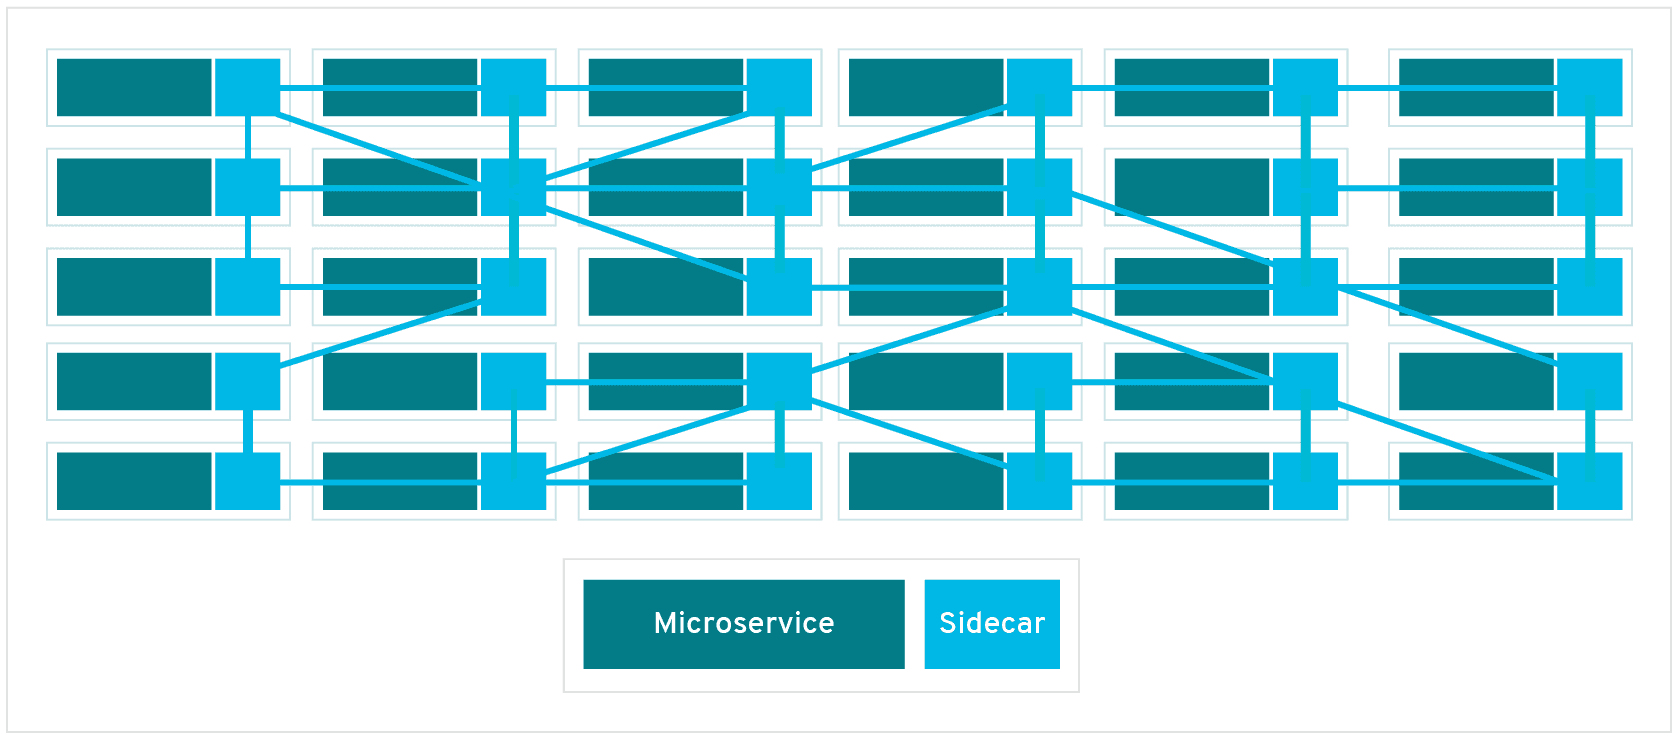
\includegraphics[width=\textwidth]{serviceMesh}
\end{center}
Minden szolgáltatás egy mikroszolgáltatásból és egy sidecar proxy-ból áll.
Mikroszolgáltatás alatt az alkalmazás egy adott funkciójának megvalósítását
valamilyen nyelven értjük. Fontos kihangsúlyozni, hogy nem kötött milyen
programozási nyelven van az adott mikroszolgáltatás írva, mert ez is
nagyon rugalmassá teszi az ilyen fejlesztést, abban az esetben, ha
különböző csapatoknak más és más nyelven akarnak megírni egyes szolgáltatásokat.
Viszont itt jön képbe a sidecar proxy, ami elvégzi az a hálózati
kommunikációt a szolgáltatások között. Szóval nem kell a fejlesztőnek
a mikroszolgáltatásban azzal foglalkozni, hogy kiknek címezze a kimenő
forgalmat vagy, hogy honnét kapja, mert ez mind a két esetben a sidecar lesz.

A kép forrása és további érdekes információk megtalálhatóak még a Red Hat ezen
cikkében ~\cite{redhat}

\subsubsection{Envoy}
Ez egy L7 (alkalmazás) rétegen működő proxy és kommunikációs csatorna
arra tervezve, hogy nagy szolgáltatás alapú architektúrákat lehessen létrehozni
úgy, hogy a szolgáltatások számára a hálózat átlátszó legyen.
A proxy egy olyan szerver, amely hálózati forgalmat irányítja. Az előzőleg
említett funkcióját úgy sikerül ellátnia, hogy a szolgáltatáshálók
részben lévő szolgáltatásoknál az Envoy lesz maga a sidecar, így a
mikroszolgáltatásnak elég mindig csak a localhost-ra küldeni és onnét
fogadni adatot.

Képes L3/L4 (hálózati/szállítási) réteg szűrőket is alkalmazni, amivel a
különböző protokollokat, mint a TCP (Transmission Control Protocol) és az
UDP.

Ezen felül rendelkezik még olyan funkciókkal, amelyek segítségével
megvalósítható perem proxy-ként és belső proxy-ként is, felügyelhető,
és HTTP (HyperText Transfer Protocol) alapú szűrést is tudunk használni.

További információk ezen az oldalon találhatóak ~\cite{envoydoc}

\subsubsection{További technológiák, amelyek szükségesek}
\textbf{UDP - User Datagram Protocol} \\
Az UDP egyszerű kapcsolatmentes összeköttetést hoz létre 2 eszköz
között, így nincs kapcsolat ellenőrzés, mint a TCP-nél ezért sokkal
gyorsabban felállítható a kapcsolat eszközök között. Viszont nincs
garancia arra, hogy a csomagok megérkeznek, sorrendben érkeznek-e
vagy, hogy duplikált csomagok jönnek át a csatornán. Ezért olyan
szolgáltatásokhoz érdemes használni, ahol nem probléma, ha egy
csomag többször jön vagy hiányoznak csomagok. Ilyenek például a
telekommunikáció és az élő közvetítések is. További információk
találhatóak ezen az oldalon ~\cite{udpwiki} \\

\textbf{UDS - Unix Domain Socket} \\
Arra használatos, hogy a folyamatok úgy tudjanak egymással kommunikálni,
hogy az minél jobb legyen. A Unix Domain Socket lehet névtelen, vagy
hozzárendelve egy fájlrendszerben létrehozott elérési útvonalhoz.
További információkat lehet találni ezen az oldalon ~\cite{udsman} \\

\textbf{iPerf} \\
Az iPerf egy olyan eszköz, amellyel lehet mérni a maximálisan elérhető
sávszéllességet IP hálózatokban. Támogatja a különböző protokollokat, így
használható TCP és UDP mérésre is, de ezen felül lehet még sok máshoz is használni.
De betudunk állítani olyanokat is, hogy adott ideig és időközökkel küldjön
általunk megadott csomagmérettel és küldési sebességgel, szóval egy
nagyon kis hasznos eszköz.

Minden ilyen teszt végén kapunk egy jelentést arról, hogy milyen sávszélességgel
érkeztek meg a csomagokat, ebből mennyi veszett el és még más paramétereket is
annak tükrében, hogy milyen részletes jelentések szeretnénk látni.

A használata úgy néz, hogy létre kell hozni egy úgynevezett iPerf szervert,
amihez beérkeznek a csomagok. Ez lehet bárhol, amit az hálózaton keresztül elérünk.
Ezen felül még létre kell hozni egy iPerf klienst is, aki az általunk
specifikált módon fog csomagokat küldeni a szerverre.

További érdekes információk találhatóak az weboldalán ~\cite{iperf} \\

\textbf{socat} \\
A Socat egy parancssori alapú segédprogram, amely két kétirányú bájt-folyam
hoz létre és adatot továbbít közöttük. Mivel az adatfolyamok különféle típusú
adatgyűjtőkből és forrásokból állíthatóak össze, és mivel sok címbeállítási
lehetőséget lehet alkalmazni az adatfolyamokra, a socat felhasználható
többféle célra.

Ezt fogjuk arra használni, hogy UDS csomagokat alakítsunk át UDP csomagokká.
További információk találhatóak a következő oldalon ~\cite{socat}
%Amikor a tágabb tudományos vagy műszaki környezetről beszélünk, akkor
%azt értjük alatta, hogy ,,művelt laikus'' -- alapesetben ennek
%tekinthető a tárgyfelelős -- megtalálja azokat a kapcsolódási
%pontokat, amelyek segítségével az ő ismereteihez a beszámolóban
%tárgyalt témakör és az elvégzett munka csatlakoztatható.  Ez
%mindenképpen, szükséges, hiszen enélkül az olvasónak előzetes
%tájékozódást kellene végeznie a szűkebb szakterületen, hogy az
%elvégzett munka jellegét, súlyát, nehézségét meg tudja ítélni.

%Természetesen a terjedelmi korlátok miatt nem lehet teljes mértékben
%bemutatni az adott szűkebb szakterületet, ezért meg kell adni az
%érdeklődő olvasónak a lehetőséget a további tájékozódásra.  Részben
%erre szolgálnak a hivatkozások\footnote{A másik nagyon fontos céljuk
%  az állítások alátámasztása.  A lábjegyzetek használatát egyébként
%  nem érdemes túlzásba vinni, mert állandóan megtörik az olvasás
%  folyamatát (lásd például \cite{esterhazy}).  Akkor kell használni,
%  amikor a lábjegyzetben közlendő információ érdekes lehet, de nem
%  tartozik közvetlenül a tárgyhoz.  Mindenképpen kerülendő az irodalmi
%  hivatkozások lábjegyzetben való megadása.}, lábjegyzetek.

%Nagyon fontos, hogy abban az esetben, amikor a hallgató féléves
%munkájának egy része vagy egésze az, hogy tanul, hogy maga is
%ismerkedik azzal a szakterülettel, amelyen dolgozni fog, akkor az
%tudatosan törekedjen arra, hogy az Elméleti összefoglaló és az
%Elvégzett munka ismertetése szétválasztható legyen.  Az előbbinek a
%szakterület alapvető, általános ismereteit kell tartalmaznia,
%amelyekről a ,,művelt laikusnak'' részleges ismeretei lehetnek.  Míg
%az elvégzett munka leírásába azoknak a specifikus ismereteknek a
%bemutatása kerülhet, amelyek a később elvégzett vagy elvégzendő
%feladatokat konkrétan megalapozzák.

%További tanulmányozásra ajánljuk Eco professzor művét~\cite{eco}.

%A hivatkozások kezelésénél fontos, hogy mindig a mondat részeként
%tekintsünk rá, és ha szükséges, akár többször is hivatkozzunk meg egy
%forrást, de az első előfordulásakor mindenképpen.  Ugyanez érvényes a
%rövidítésekre: minden rövidítést a legelső előforduláskor magyarázni
%kell, később viszont használhatók a rövidített formák is.  Például: a
%Tiger Tree Hash (TTH) a hashelés egy speciális formája.

\subsection{A munka állapota, készültségi foka a félév elején}
\label{sec:munka-allap-kesz}
A témalaboratórium alkalmával már foglalkoztam a szolgáltatáshálók
megismerésével és használatával, ahol az Isio és az SMI (Service Mesh
Interface) különböző aspektusait hasonlítottam össze. Ennek során
mélyebb rálátást sikerült nyernem a Kubernetes használatára és arra,
hogy egy jó dokumentáció milyen nagy segítséget nyújthat azoknak,
akik ebben az iparágban dolgoznak.
%Ebben a részben lehet megadni a korábbi félévekben elvégzett munkát
%is.  Így világosan elkülöníthető az aktuális félévtől.  Nem kell
%hosszasan írni, de ne legyen felsorolás sem.  Egy bekezdésben kellene
%itt leírni, hogy foglalkoztál-e már ezzel a témával, a tanszéken
%dolgozott-e már valaki rajta.  Írd le azt is, hogy mit kaptál kézhez
%hozzá segítségként.

\newpage
%==================================================================
\section{Az elvégzett munka és az eredmények ismertetése}
\label{sec:az-elvegzett-munka}


\subsection{A munkám ismertetése logikus fejezetekre tagoltan}
\label{sec:a-munkam-ismert}
Minden konfiguráció, amit a labor során elvégeztem statikusan működik, vagyis
csak egy megadott IP cím és port párosra érvényesek, amelyeket meg kell adni a
konfigurációs fájlokban. Később a szakdolgozatban szeretném majd úgy
megvalósítani ezeket a feladatokat, hogy dinamikusan tudjanak működni.
\subsubsection{Lokális környezet}
Minden konfigurációt és mérést Ubuntu 18.04 LTS (Long Term Support) környezetben
végeztem el, annak érdekében, hogy konzisztensebb legyen a mérés a későbbiekben is,
mert számomra egyszerűbb dockert és kubernetest használni Linux alapú környezetben,
mint Windows-ban.

Ahhoz, hogy lokálisan, docker és kurbernetes nélkül tudjam használni az Envoy-t
elsőnek is telepíteni kellett, amit a Lyft (akik az Envoy-t fejlesztik) által
nyújtott dokumentáció alapján sikerült, viszont egy külső forrás alapján nagyon
egyszerűen megvalósítható volt. Ennek a részleteibe nem szeretnék belemenni, mert
csak utasításokat kell követni, viszont ezen az oldalon megtalálhatóak ~\cite{envoylocal}.

Ehhez és a másik két környezethez is az Envoy legújabb verzióját használtam, ami a
1.14.1-s verziószámot jelenti.

Ahhoz, hogy a proxy-t lehessen konfigurálni YAML (YAML Ain't Markup Language)
fájlt/fájlokat kell létrehozni. Ezeket a fájlokat adattárolásra és konfigurációk
létrehozására szokás használni, mert könnyű őket olvasni és írni is.

Esetünkben három része lesz, ennek a fájlnak, amire oda kell figyelni és módosítani.
Ezek lesznek azok a részek: \textbf{admin, listeners, clusters}. Az Envoy
dokumentációjában találtam egy példa fájlt, amit alapnak vettem minden alkalommal,
ez a fájl megtalálható ezen az oldalon ~\cite{envoyudpconf}

Az admin rész csak annyiban érdekes számunkra, hogy a 127.0.01:9901-s címen
ezáltal elérjük az általunk beállított porxy konfigurációját, logjait és hasonló
értékeket, de ezek megtalálhatóak lokálisan is, ahol fut az Envoy. Mivel a
kezelőfelületnek nem kell feltétlen UDP alatt működnie így az maradhat TCP is.

Ezután közvetlen jön a Listeners, mint a neve is utal rá, ami ez alatt a blokk
alatt fog szerepelni, olyan attribútumú csomagokra fog figyelni. Elméletileg
egy ilyen konfigurációban megadható egynél több listener is, de ezt nem ajánlják
az Envoy dokumentációjában, mert úgy nehezebb karbantartani és statisztikai adatokat
kinyerni. Mivel csak lokálisan fog futni a proxy, ezért localhost-on fogunk figyelni
és annak egy általunk választott portján, aminek én most a \textbf{4000}-set választottam.
Fontos ugye az is, hogy itt már UDP csomagokra kell figyelnünk, ami azt jelenti,
hogy erre a címre érkező csomagok csak UDP protkollal rendelkezhetnek. Fontos
még, hogy a listener-en belül még be legyen állítva ez az érték is:
\textbf{reuse\_port: true}, mert alapértelmezetten az Envoy nem hoz létre socket-et
minden a dolgozó szálaknak, így viszont kitudjuk kényszeríteni, hogy minden
ilyen szálnak legyen egy sajátja.

Legutolsó sorban a Klaszter rész jön, ahol statikusan beállítjuk, hogy milyen címre
továbbítsa azokat a csomagokat, amit a listener-ben beállítottunk. Ezt én most
a 127.0.0.1:5000 címre állítottam be, aminek a portszámát kedvünk szerint módosíthatjuk,
de oda kell figyelni arra, hogy ez ne egyezzen a konfiguráció során beállított más
porttal, mert akkor sajnos nem fog működni a továbbítás. Ezen felül több
végpontot is megadhatunk nem csak egyet így megoldható a terhelés elosztás is
különböző pontok között. Ebben az esetben elég számunka az alap ROUND\_ROBIN,
ami elméletileg sorra haladna végpontokon és sorban küldené ki a csomagokat, de
mivel nálunk csak egy végpont lesz így ezt nem fogjuk tapasztalni.

A kész konfigurációs fájl megtalálható lesz, a csatlakozó dokumentumok jegyzékénél.

A konfigurációnkat már csak el kell fogadtatni az Envoy-al, hogy aszerint
fogadja és továbbítsa a bejövő forgalmat. Ezt egy egész egyszerű paranccsal
megtudjuk tenni: \textbf{envoy -c <s fájl elérési útvonala>}

Ezután már nem marad más csak tesztelni, hogy milyen sávszélességgel képes
továbbítani a csomagokat. Ennek a mérésére fogjuk használni az iPerf parancsot.

Az iperf szervert a következő paranccsal hozzuk létre.
\begin{center}
  \begin {verbatim}
     iperf -s -p 5000 -u -U -e -i 1 --realtime
  \end{verbatim}
\end{center}
Ezzel megadtuk, hogy az 5000-s porton figyeljen UDP forgalomra és csak egy UDP
szálon figyelünk. Az -e kapcsoló felel azért, hogy részletesebb adatokat kapjunk,
mindezt másodpercekre bontva valós időben.

Ezután létre kell hozni az iperf klienst is, aki a forgalmat fogja biztosítani.
\begin{center}
  \begin{verbatim}
    iperf -u -c 127.0.0.1 -p 4000 -b 72250000 -l 100 -i 1 -t 10
  \end{verbatim}
\end{center}
UDP forgalmat továbbítunk a 120.0.0.1:4000-s címre, ugye ezen figyel az
általunk beállított proxy. 72.3 Mbit/s sebességgel 100 byte-os csomagokkal
másodpercenként küldjük a csomagokat 10 másodpercen keresztül.

A teszt eredménye a szerveroldalon lesz látható.

Ez még kellene.
\subsubsection{Dockeres környezet}
A dockeres megvalósításnál is igazából hasonlóan fogunk eljárni, mint lokálisan, de
csak annyi fog különbözni, hogy nem a mi számítógépünk fog futni, hanem a konténerben.
Ez azért egy jó megoldás, mert így akár több ilyen proxy is könnyedén létrehozható
más és más konfigurációkkal. \\

Ahhoz, hogy ezt megtudjuk valósítani elsőnek a Docker egy vverzióját kell
telepítenünk. Telepítésnél oda kell figyelni, hogy Snap store-ból nem szabad,
mert, akkor nem fog minden funkcionalitása megfelelően működni. Telepítés
folyamatát érdemes Docker által nyújtott dokumentáció alapján csinálni ~\cite{installdocker}.

Ha már van Docker a gépünkön, akkor elsőnek le kell tölteni a megfelelő Envoy
képfájlt a DockerHub-ról, amit a következő paranccsal egyszerűen megtehetünk.
\begin{center}
  \begin{verbatim}
    sudo docker pull envoyproxy/envoy:v1.14.1
    sudo docker images
  \end{verbatim}
\end{center}
Az első paranccsal az általunk kívánt képfájl és adott verziója fog letöltődni,
míg a másodikkal ellenőrizni tudjuk, hogy megvan-e a képfájl.

Ezután már csak a konfigurációs YAML fájlt kell megcsinálni, ami nagyon hasonló
lesz, mint a lokálisnál, csak annyiban fog különbözni, hogy nem localhost-ról
fogunk csomagokat kapni és nem is oda fogunk küldeni, hanem a docker konténer
saját IP címére fogunk. Ez a cím nekem a \textbf{172.17.0.1}, de a \textbf{ip a}
paranccsal könnyen ellenőrizni tudjuk. De minden más marad a régiben.

Ahhoz, hogy ezt a konténert létre tudjuk hozni a következő parancsot kell kiadni:
\begin{center}
  \begin{verbatim}
    docker run --net=host --name=proxy-udp -d \
    > -p 9901:9901 \
    > -p 4000:4000 \
    > -v $(pwd)/udpDocker.yaml:/etc/envoy/envoy.yaml \
    > envoyproxy/envoy:v1.14.1
  \end{verbatim}
\end{center}
Az elsősorban megadjuk, hogy milyen hálózatban legyen a konténerünk, aminek most a
kiszolgáló hálózata lett beállítva és adtunk neki egy kicsit jobban megjegyezhető
nevet, mint amit egyébként a docker adna neki. Az utána következő 2 sorban azt
a két portot adjuk meg, amelyeken keresztül a konténerünk elérhetővé válik. Utána
jön az izgalmasabb rész, ahol az általunk írt konfigurációs fájl tartalmát betöltjük a
konténerben lévőbe. Ezt azért kell megcsinálni, mert az alapképfájlban van egy
alapkonfiguráció, ami jelenleg számunkra nem kell szóval felül kell írni.
Másrészt, azért is szükség van arra, hogy így megadjuk, mert így nem kell a
konténerbe belépni, majd ott megadni a fájlt, ami esetleg több ilyen konténer
létrehozásánál elég fárasztó lehet. Az utolsó sornál pedig csak a képfájl nevét
adjuk meg elérhetőségnek.

A sebesség mérése csak annyiban fog különbözni az előzőhöz képest, hogy nem a
127.0.0.1:4000-s címre fogunk csomagokat küldeni, hanem a 171.17.0.1:4000 címre.\\

Ehhez a részhez tartozó konfigurációs fájl is megtalálható a csatlakozó
dokumentumok jegyzékében.

Itt is meg kell csinálni a sebességmérést.
\subsubsection{Kubernetes környezet}
Ahhoz, hogy kubernetes-ben is létre tudjuk hozni ugyan ezt a környezetet, ahhoz kell
egy olyan program amellyel virtuális létre tudunk hozni egy dolgozó node-t.
Erre tökéletes lesz a Minikube, de ahhoz hogy ezt tudjuk használni kell, hogy
a számítógépünk képes legyen virtualizációra. Virtualizálni a legtöbb
gép már képes, de ha virtuális környezetben dolgozunk, akkor azok nem képesek arra.
Mindemellet kell, hogy legyen valamilyen eszköz, amely az alapot fogja
biztosítani a Minikube-nak. Én a VirtualBox-t választottam, amiben
virtuális gépeket lehet létrehozni, de ez lehetett volna VMware vagy KVM is.

A Minikube és a Kubernetes könnyedén telepíthető a következő oldal
segítségével ~\cite{installkubectl}

Mivel most nem egy nagy erőforrás igényű alkalmazást fogunk létrehozni nem
kell a virtuális gép paramétereit beállítani és elég csak szimplán indítani a
Minikube-t a következő paranccsal.
\begin{verbatim}
  minikube start
\end{verbatim}
Így 2 CPU maggal, 2 GB memóriával és 20 GB tárhellyel fog létrejönni. Szükséges
megjegyeznünk a későbbiekhez az ip címét.
\begin{verbatim}
  minikube ip
  192.168.99.100
\end{verbatim}
Ezután létre kell hoznunk a saját Envoy képfájlunkat, mert ha az alap
fájlból szeretnénk létrehozni a pod-ot, akkor nem fogjuk tudni úgy
konfigurálni, ahogyan azt mi szeretnénk. Ahhoz, hogy ezt megtudjuk csinálni
írnunk kell egy \textbf{Dockerfile}-t, amiben specifikáljuk, hogy mi legyen az
alap képfájl, milyen konfiguráció legyen beállítva és, hogy milyen parancs
fusson le a konténer létrejöttekor. Így néz ki a Dockerfile:
\begin{verbatim}
  FROM envoyproxy/envoy:v1.14.1
  COPY envoy_upd.yaml /etc/envoy/envoy.yaml
  RUN apt-get update && apt-get install -y tcpdump && apt-get install -y net-tools
\end{verbatim}
Mint látszik, az első sorban az alap képfájlt adjuk, meg míg a másodikban a
saját konfigurációnkat bemásoljuk, abba a fájlba, amiből dolgozni fog az Envoy,
mihelyt elindul. Az utolsó sor már csak, azért kell, hogy esetleges hibákat
egyszerűbb legyen kideríteni és megoldani.

Most létre kell hozunk a YAML fájlt, ami nagyon hasonlítani fog az előzőekhez,
viszont annyiban el fog térni, hogy itt már bármilyen címről érkező UDP csomagot
el fogunk fogadni, ha az 5000-s portról érkezik. Viszont küldeni egy címre fogunk
csak, ami az én esetemben a VirtualBox által létrehozott lesz, ami 192.168.99.1.
Ezt könnyen kideríthető az \textbf{ip a} paranccsal.

Miután mindez megvan, már csak létre kell hozni az általunk megadott képfájlt és
azt feltölteni a DockerHub-ra, ahonnét majd később le fogjuk tudni tölteni.
\begin{verbatim}
  sudo docker build .
  sudo docker tag <image_id> vidarhun/kubeudpenvoy:v1
  sudo docker push vidarhun/kubeudpenvoy:v1
\end{verbatim}
Most egy Deploymentet fogunk létrehozni, amire azért van szükség, mert így
a Pod véletlenszerű törlődése esetén rögtön létre fog jönni egy ugyan olyan
funkcionalitású, de más IP-vel rendelkező Pod. De ugyanakkor később, ha több
ilyen Pod-ra lenne szükségünk, akkor a számukat könnyen fel lehet skálázni
annak megfelelően, hogy mennyi terhelése érkezik a szolgáltatásunkba.
A legfontosabb részét bemutatom és részletesen ismertetem, de ez a fájl is
megtalálható lesz csatlakozó dokumentumok jegyzékében.
\begin{verbatim}
  spec:
    containers:
    - name: envoy-container
      image: vidarhun/kubeupdenvoy:v1.0
      ports:
        - containerPort: 5000
          protocol: UDP
\end{verbatim}
Itt állítjuk be, hogy a Podunk milyen névvel jöjjön létre és, hogy az
általunk létrehozott és felöltött képfájl alapján jöjjön létre.
Fontos még az, hogy a konténernek egyezzen a nyitott portja a konfigurációs
fájlban a listener-nél megadott porttal, mert így lesz képes a csomag betalálni
hozzá. A kimenő forgalom számára, azért nem kell ilyen pontosan specifikálni,
mert a Pod teljes mértékben képes kilátni a klaszterből és a VirtualBox
csatlakozási pontját megtalálni.

valami 
% <Én magam (nem a társam) a félév során következőket olvastam el /
% programoztam / készítettem el / teszteltem / dokumentáltam / néztem át
% / tanultam meg, stb.  Tételes leírása és felsorolása mindannak, ami a
% félév során történt, alátámasztandó azon állításom a
% konzulens/tárgyfelelős felé, hogy összességében mindent beleértve
% tényleg dolgoztam a TVSZ szerint kreditenként 30 órát, azaz a heti 2
% kontakt órás tárgy esetében min. $2,5*30 = 75$ munkaórát, illetve a
% heti 6 kontakt órás tárgy esetében min. $8*30 = 240$ munkaórát\dots>
%
% Ebben a részben a hallgató az általa elvégzett munkát mutatja
% be. Hangsúlyosan a saját munka bemutatása a cél, hiszen a hallgató
% ezzel igazolja a témavezető és a tárgyfelelős irányába, hogy --
% folyamatosan fejlődve és egyre több és jobb munkát végezve -- a
% szakdolgozatát/diplomadolgozatát képes lesz megírni.  A beszámoló nem
% munkanapló, nem arra vagyunk kíváncsiak, hogy mit mikor csinált a
% hallgató és mennyi időt töltött vele, hanem egy eredmény-centrikus
% beszámolót szeretnénk olvasni.  De itt is fontos tudni, hogy
% megosztott feladat esetén ki-mit csinált, mekkora részt vállalt.
%
% Az egész beszámoló elkészítésénél törekedni kell a magyar nyelv
% szabályainak követésére és a műszaki dokumentáció/tudományos közlemény
% írásával kapcsolatosan kialakult közmegegyezés szerinti formai
% követelmények betartására.  (Tehát nem kell többes számként hivatkozni
% saját magunkra, kerülni kell a furcsa megfogalmazást, passzív és egyéb
% kifacsart mondatszerkezeteket.  Az egy szót határozatlan névelőként
% történő használatakor ne írjuk ki számként.)
%
%
% A beszámoló természetesen nem csak szöveget tartalmazhat, hanem
% képleteket, táblázatokat, ábrákat és még sok minden mást.  Ezek
% kapcsán az alábbi elvek irányadók:
% \begin{itemize}
% \item Az ábráknak, képeknek és táblázatoknak mindig van számuk és
%   címük. (A cím nem ennyi: ,,1. ábra'', hanem azt írd le, ami látható
%   rajta.)
%
% \item Az ábrákra, a képekre és a táblázatokra a szövegben hivatkozni
%   kell, és a szövegben elemezni kell azokat. Például
%   \aref{fig:fig1}.~ábrán látszik, hogy a vizsgált félévben még két
%   napos csúszással is lehetett jeles érdemjegyet szerezni a tárgyból,
%   de a pontosság még nem garancia a jó jegyre: öten nem kaptak jelest,
%   noha nem késtek a leadással.
%
% \item Az ábrák, képek és táblázatok mérete a szükségesnek megfelelő
%   legyen: elég nagy ahhoz, hogy kinyomtatva is olvasható és
%   értelmezhető legyen, de nem nagyobb annál, mint amit szerepe
%   indokol.
%
% \item A grafikonoknak a tengelyeken legyenek feliratai és ha releváns,
%   a mértékegység is.
%
% \item A képletek esetében nem minden képletre történik hivatkozás, de
%   ahol igen, ott a képletet a műszaki irodalomban jellemző módon a sor
%   végére tett kerek zárójelben lévő számmal jelöljük meg.  A
%   képleteket ne képként illeszd be a szövegbe.
%
% \item Kódrészleteket, ha nem relevánsak, ne illeszd be képként, főleg
%   ne rossz minőségben. Nyugodtan teheted függelékbe és hivatkozd be a
%   szövegben, mint a képeket, például: Az 1.~számú függelékben
%   található az adatbeolvasó kód, melyet C++ nyelven készítettem el.
% \end{itemize}
%
% Az írásbeli beszámolót a témavezető és a tárgyfelelős is értékeli. A
% tárgyfelelősi értékelés szempontjai az alábbiak:
% \begin{enumerate}
% \item Megfelel-e az elvégzett munka a félév elején kiadott feladatnak?
% \item Megfele-e a beszámoló a formai követelményeknek? Ezen belül:
%   \begin{itemize}
%   \item a. Megfelelő-e az elméleti bevezető és az irodalomjegyzék?
%   \item b. Egyértelmű-e, hogy mi volt a hallgató saját munkája?
%   \item c. Megfelelő-e a dokumentum technikai színvonala?
%   \end{itemize}
%
% \end{enumerate}
% Ezen kívül a tárgyfelelős veszi figyelembe az értékelés során
% kialakult félévi jegyre vonatkoztatva az ún. ,,hanyagsági faktor''
% értékét, amelyet (\ref{eq:1}) szerint állapítunk meg:
%
% \begin{equation}
%     F_{hany} = 1 - a - b
%   \label{eq:1}
% \end{equation}
%
%
% \begin{figure}[tbh]
%   \centering
%   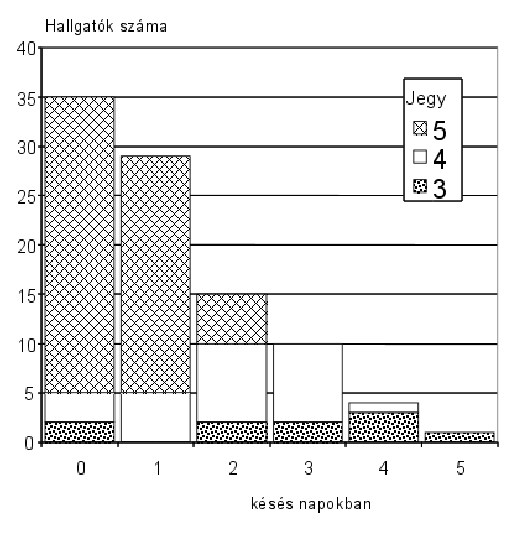
\includegraphics[]{fig1.eps}
%   \caption{Hallgatók érdemjegyeinek eloszlása az írásbeli beszámoló késése függvényében}
%   \label{fig:fig1}
% \end{figure}
%
% Az (\ref{eq:1})-ben szereplő a szám a munkaterv beadásában történt
% késedelemre, míg a b szám az írásbeli beszámoló beadásában történt
% késedelemre vonatkozik.  Utóbbi értékeiről
% \aref{tab:hanyagsagi}.~táblázat tájékoztat.
%
% \begin{table}
%   \centering
%     \begin{tabular}{|l|c|}
%       \hline
%       Az írásbeli beszámoló beadásának napja     & A ,,b'' faktor értéke \\
%       a szóbeli beszámolóhoz képest (munkanapban) & ~ \\ \hline
%       -4.~munkanap & $0.04$ \\ \hline
%       -3.~munkanap & $0.09$ \\ \hline
%       -2.~munkanap & $0.20$ \\ \hline
%       -1.~munkanap & $0.30$ \\ \hline
%       \end{tabular}
%     \caption{Az írásbeli beszámoló késedelmes beadásával kapcsolatos hanyagsági faktor értéke}
%   \label{tab:hanyagsagi}
% \end{table}
%
% A beszámoló értékeléséről részletesebben írunk \cite{web}-ban.
%
% A beszámolóban bizonyára szerepelni fognak rövidítések. Ezeket a
% rövidítéseket, betűszavakat néhány, az infokommunikáció területén
% nagyon ismert és gyakran használt kifejezéstől (például IP, TCP, GPRS,
% UMTS) eltekintve ki kell fejteni logikusan az első használat
% alkalmával (például így: ,,A GPS (Generalized Processor Sharing) egy
% ideális folyadékmodellen alapuló csomagütemező eljárás.'').
%
% A beszámoló készítése során előfordulhat, hogy a hallgató úgy érzi,
% hogy alfejezetekkel tagolva jobban olvasható és érthető lenne a
% beszámoló.  Ennek akadálya nincs, de érdemes arra figyelni, hogy a
% túlzott tagolás sem tesz jót egy írásműnek, illetve hogy a címsorokban
% a rövidítések és a hivatkozások használata tilos.  Tartalomjegyzéket
% készíteni nem szükséges a beszámolóhoz, de nem is tilos, kivéve azt az
% esete, amikor nyilvánvalóan terjedelemnövelési célokat szolgál.
%
% A beszámoló terjedelme tárgyanként változhat.  Általános szabály, hogy
% 1 hüvelyknél nagyobb margókat ne használjunk.  A szöveg legyen
% egyszeres sortávú, sorkizárt és 12 pontos betűméretű.  A bekezdések
% kezdődjenek behúzással a minta szerint.

\subsection{Összefoglalás}
\label{sec:osszefoglalas}

A félévi munka során elért új eredmények ismételt, vázlatos, tömör
Ebben a részben az adott félévre vonatkozó, az \emph{Önálló
  laboratórium tárgy keretében elvégzett munka során} elért
\textbf{új} eredmények ismételt, vázlatos, \textbf{tömör}
összefoglalását várjuk, lehetőleg nem felsorolásként.  Itt még egyszer
ki lehet térni a leglényegesebb eredményekre, valamint a félév során
felmerülő nehézségekre, de meg lehet említeni a továbbfejlesztési
irányokat, lehetőségeket is.

Ezt a részt tagolható a következő pontok megválaszolásával:
\begin{itemize}
\item Mi volt az \textbf{aktuális kérdés}, probléma, amivel a félév
  során foglalkoztál?
\item Mi a dolgozat \textbf{célja}, miért érdekes egyáltalán ezzel a
  problémával foglalkozni?
\item Milyen \textbf{módszereket} használtál a probléma megoldása
  érdekében?
\item Mik a legfontosabb \textbf{eredmények}?
\item Milyen \textbf{következtetéseket} lehet levonni?

\end{itemize}

Ha valaki elolvassa ezt a részt, képet kell kapnia az egész
dolgozatról.  Ne legyen az absztrakt szó szerinti ismétlése.

Fontos, hogy az itt megadott sablontól el lehet térni, használata nem
kötelező, csak segítséget jelenthet, viszont a fedőlap lehetőleg
maradjon ugyanez és tartalmilag egyezzen meg a sablon irányelveivel. A
beszámoló felépítésében nem érdemes eltérni a \emph{Bevezető --
  Féléves munka és eredmények bemutatása -- Összefoglaló} hármastól.

\newpage

%==================================================================
\section{Irodalom, és csatlakozó dokumentumok jegyzéke}
\label{sec:irod-es-csatl}

\begin{thebibliography}{9}
\label{sec:tanulm-irod-jegyz}

\bibitem{linuxwindows} Microsoft Corporation, \emph{Linux containers on Windows 10} \\
\url{https://docs.microsoft.com/en-us/virtualization/windowscontainers/deploy-containers/linux-containers}

\bibitem{dockerhub}  Docker Inc, \emph{DockerHub} \url{https://hub.docker.com/}

\bibitem{dockeroff}  Docker Inc, \emph{Docker Documentation} \url{https://docs.docker.com/}

\bibitem{dockerwiki} Wikipedia contributors, \emph{Wikipedia:Academic
    use}, Wikipedia, The Free Encyclopedia, 2011 Nov 11.  Available
  from: \\ \url{https://en.wikipedia.org/wiki/Docker_(software)}

\bibitem{minikube} The Kubernetes Authors, \emph{Minikube documentation} \url{https://minikube.sigs.k8s.io/docs/}

\bibitem{redhat} Red Hat Inc, \emph{What's a service mesh?}
\\ \url{https://www.redhat.com/en/topics/microservices/what-is-a-service-mesh}

\bibitem{envoydoc} Envoy Project Authors, \emph{What is Envoy}
\\ \url{https://www.envoyproxy.io/docs/envoy/latest/intro/what_is_envoy}

\bibitem{udpwiki} Wikipedia contributors, \emph{User Datagram Protocol}
\\ \url{https://en.wikipedia.org/wiki/User_Datagram_Protocol}

\bibitem{udsman}  Linux man-pages project, \emph{Unix Domain Socket}
\\ \url{http://man7.org/linux/man-pages/man7/unix.7.html}

\bibitem{iperf}  iPerf contributors, \emph{iPerf} \url{https://iperf.fr/}

\bibitem{socat}  Gerhard Rieger, \emph{socat - Linux man page} \url{https://linux.die.net/man/1/socat}

\bibitem{envoylocal} ComputingforGeeks - Home for *NIX Enthusiasts, \emph{How To Install Envoy Proxy on Ubuntu / Debian Linux} \\
\url{https://computingforgeeks.com/how-to-install-envoy-proxy-on-ubuntu-debian-linux/}

\bibitem{envoyudpconf} Envoy Project Authors, \emph{UDP proxy} \\
\url{https://www.envoyproxy.io/docs/envoy/v1.14.1/configuration/listeners/udp_filters/udp_proxy}

\bibitem{installdocker}  Docker Inc, \emph{Docker Documentation}
\\ \url{https://docs.docker.com/engine/install/ubuntu/}

\bibitem{installkubectl} The Kubernetes Authors, \emph{Install Minikube}
\\ \url{https://kubernetes.io/docs/tasks/tools/install-minikube/}

\bibitem{web} \emph{Tájékoztató a Műszaki Informatika Szak önálló
    laboratórium tantárgyainak 2008/9. tanév I. félévi lezárásáról a
    BME TMIT-en (VITMA367, VITMA380, VITT4353, VITT4330),}
  \url{http://inflab.tmit.bme.hu/08o/lezar.shtml}, szerk.: Németh Felicián,
  2008. november 5.

\bibitem{wikipedia} Wikipedia contributors, \emph{Wikipedia:Academic
    use}, Wikipedia, The Free Encyclopedia, 2011 Nov 11.  Available
  from: \\ \url{http://en.wikipedia.org/w/index.php?title=Wikipedia:Academic\_use\&oldid=460041928}

\end{thebibliography}

Itt jegyezném meg, hogy a tanulmányozott irodalmat hivatkozni kell a
szövegben.  Szükség esetén többször is.  Az irodalomjegyzék célja
(lásd \aref{sec:tanulm-irod-jegyz} fejezetet) ugyanis
kettős\footnote{Akárcsak ennek a fejezet hivatkozásnak, ami a
  \texttt{$\backslash$aref babel} parancsot demonstrálja}:
\begin{enumerate}
\item Az olvasó tájékoztatása, hogy a dokumentumban ki nem fejtett
  dolgoknak, a tudottnak vélt ismereteknek hol lehet bővebben
  utánanézni, így ott kell meghivatkozni az irodalmat~\cite{eco,
    esterhazy}, ahová az irodalom kapcsolódik.
\item Megmutatni a tárgyfelelosnek/konzulesnek az elolvasott irodalom
  mennyiségét
\end{enumerate}

Javasoljuk, hogy a hallgatók tanulmányozzák, hogyan néznek ki a
hivatkozások a villamosmérnöki/informatikai szakma vezető szakmai
folyóirataiban megjelenő cikkekben.  Ebben a témavezető is biztosan
tud segíteni.  A hivatkozás teljességére és egyértelműségére tessék
ügyelni.  Például, ha egy könyvnek több, eltérő kiadása is van, akkor
azt is meg kell jelölni, hogy melyik kiadásra hivatkozunk.  A webes
hivatkozások problémásak szoktak lenni, de manapság egyre több az
olyan dokumentum, ami csak weben lelhető fel, ezért használatuk nem
zárható ki. Itt is törekedni kell azonban a pontosságra és a
visszakereshetőségre. A weben található dokumentumoknak is van címe,
szerzője, illetve érdemes megadni a letöltés/olvasás időpontját is,
hiszen ezek a dokumentumok idővel megváltozhatnak.

A wikipédiás hivatkozások használata nem javasolt, mert a wikipedia
másodlagos forrás.  Tájékozodjuk a wikipédián, de aztán olvassuk el az
adott oldalhoz megadott hivatkozásokat is.  A wikipedián külön szócikk
foglalkozik azzal, hogy miért nem szerencsés tudományos munkákban a
wikipédiára hivatkozni \cite{wikipedia}.

Nem publikus dokumentumok hivatkozása nem javasolt és csak kivételes
helyzetben elfogadható!

%==================================================================
\subsection{A csatlakozó dokumentumok jegyzéke}
\label{sec:csat-irod}

Lokális környezet konfigurációs fájlja.
\begin{verbatim}
  admin:
    access_log_path: /tmp/admin_access.log
    address:
      socket_address:
        protocol: TCP
        address: 127.0.0.1
        port_value: 9901
  static_resources:
    listeners:
    - name: listener_0
      reuse_port: true
      address:
        socket_address:
          protocol: UDP
          address: 127.0.0.1
          port_value: 4000
      listener_filters:
        name: envoy.filters.udp_listener.udp_proxy
        typed_config:
          '@type': type.googleapis.com/envoy.config.filter.udp.udp_proxy.v2alpha.UdpProxyConfig
          stat_prefix: service
          cluster: service_udp
    clusters:
    - name: service_udp
      connect_timeout: 0.25s
      type: STATIC
      lb_policy: ROUND_ROBIN
      load_assignment:
        cluster_name: service_udp
        endpoints:
        - lb_endpoints:
          - endpoint:
              address:
                socket_address:
                  address: 127.0.0.1
                  port_value: 5000
\end{verbatim}

Dockeres környezet konfigurációs fájlja.
\begin{verbatim}
  admin:
    access_log_path: /tmp/admin_access.log
    address:
      socket_address:
        protocol: TCP
        address: 127.0.0.1
        port_value: 9901
  static_resources:
    listeners:
    - name: listener_0
      reuse_port: true
      address:
        socket_address:
          protocol: UDP
          address: 172.17.0.1
          port_value: 4000
      listener_filters:
        name: envoy.filters.udp_listener.udp_proxy
        typed_config:
          '@type': type.googleapis.com/envoy.config.filter.udp.udp_proxy.v2alpha.UdpProxyConfig
          stat_prefix: service
          cluster: service_udp
    clusters:
    - name: service_udp
      connect_timeout: 0.25s
      type: STATIC
      lb_policy: ROUND_ROBIN
      load_assignment:
        cluster_name: service_udp
        endpoints:
        - lb_endpoints:
          - endpoint:
              address:
                socket_address:
                  address: 172.17.0.1
                  port_value: 5000
\end{verbatim}

<A munka ezen beszámolóba be nem fért eredményeinek (például a forrás
fájlok, mindenképpen csatolni akart forráskód részlet, felhasználói
leírások, programozói leírások (API), stb.) megnevezése,
fellelhetőségi helyének pontos definíciója, mely alapján a az
erőforrás előkereshető -- értelemszerűen nem nyilvános dokumentumok
hivatkozása nem elfogadható.>

\end{document}

%%% Local Variables:
%%% mode: latex
%%% TeX-master: t
%%% End:
